\begin{center}
    \begin{large}
    Cp 7 - It is all about The Matrix\\
    Curso \academicyear\\
    \end{large}
    \begin{figure}[h]
    	\centering
    	
\includegraphics[width=0.5\linewidth]{cp7/matrix.png}
    \end{figure}
\end{center}

% \section{Matriz}
% Implemente una clase llamada \textcolor{cyan}{Matrix} para representar el comportamiento de una matriz bidimensional. Una matriz consta de una colección de elementos distribuidos en filas y columnas.

\subsection*{Funcionalidades a implementar}
\begin{itemize}
    \item \textbf{Número de filas}: Obtener el número de filas.
    \item \textbf{Número de columnas}: Obtener el número de columnas.
    \item \textbf{Tamaño}: Obtener el total de elementos de la matriz.
    \item \textbf{Obtener un elemento}: Obtener un elemento específico de la matriz dado su índice (fila, columna).
    \item \textbf{Modificar un elemento}: Modificar un elemento específico de la matriz dado su índice (fila, columna).
    \item \textbf{Suma de matrices}: Realiza la suma de dos matrices y devuelve el resultado como una nueva matriz.
    \item \textbf{Resta de matrices}: Resta una matriz de otra y devuelve el resultado como una nueva matriz.
    \item \textbf{Multiplicación de matrices}: Multiplica dos matrices y devuelve el resultado como una nueva matriz.
    \item \textbf{Transpuesta de una matriz}: Devuelve la transpuesta de la matriz.
    \item \textbf{Multiplicación por un escalar}: Multiplica todos los elementos de la matriz por un escalar y devuelve el resultado como una nueva matriz.
    \item \textbf{Representación en cadena de caracteres}: Devuelve una cadena que representa la matriz en un formato legible.
    \item \textbf{Igualdad}: El resultado será `true` si ambas continen los mismos elementos en las mismas posiciones, de lo contrario debe evaluar `false`.
    \item \textbf{Es simétrica}: Verifica si la matriz es simétrica.
    \item \textbf{Es diagonal}: Verifica si la matriz es una matriz diagonal.
    \item \textbf{Traza de la matriz}: Calcula la traza de la matriz.
    \item * \textbf{Es ortogonal}: Determina si la matriz es ortogonal.
    \item **\textbf{Determinante de una matriz}: Calcula y devuelve el determinante de la matriz (solo aplicable a matrices cuadradas).
    \item **\textbf{Matriz inversa}: Calcula la matriz inversa (si existe).
\end{itemize}


% \section{Vector}
% Implemente una clase llamada \textcolor{cyan}{Vector} para representar el comportamiento de un vector en un espacio n-dimensional. Un vector consta de una colección de componentes.

\subsection*{Funcionalidades a implementar}
\begin{itemize}
    \item \textbf{Obtener componente}: Devuelve el valor de un componente en una posición específica del vector.
    \item \textbf{Modificar componente}: Establece el valor de un componente en una posición específica del vector.
    \item \textbf{Tamaño}: Obtener el total de elementos del vector.
    \item \textbf{Norma del vector}: Calcula la norma del vector (norma Euclídea).
    \item \textbf{Suma de vectores}: Realiza la suma de dos vectores y devuelve el resultado como un nuevo vector.
    \item \textbf{Resta de vectores}: Resta un vector de otro y devuelve el resultado como un nuevo vector.
    \item \textbf{Multiplicación por un escalar}: Multiplica todos los componentes del vector por un escalar y devuelve el resultado como un nuevo vector.
    \item \textbf{Producto punto}: Calcula el producto punto (o producto escalar) entre dos vectores.
    \item \textbf{Representación en cadena de caracteres}: Devuelve una cadena que representa el vector en un formato legible.
    \item \textbf{* Ángulo entre vectores}: Calcula el ángulo entre dos vectores.
    \item \textbf{Sistema de ecuaciones}: Implemente un método que dado una matriz A y un vector b resuelva el sistema de ecuaciones lineales $Ax = b$.
\end{itemize}


\section{Suma de matrices:}  
Implemente un método que reciba dos matrices (arrays bidimensionales de tipo entero que representan matrices algebraicas) y devuelva su suma.

\section{Multiplicación de matrices:}  
Implemente un método que reciba dos matrices (arrays bidimensionales de tipo entero que representan matrices algebraicas) y devuelva su multiplicación. Asuma que las matrices de entrada son multiplicables.

\section{Traza:}  
Implemente un método que reciba una matriz cuadrada (un array bidimensional de tipo entero que representa una matriz algebraica) y devuelva la suma de los elementos de su diagonal.

\section{Transpuesta:}  
Implemente un método que reciba una matriz (un array bidimensional de tipo entero que representa una matriz algebraica) y devuelva su transpuesta (intercambiar filas y columnas).

\section{Chequear simetría:}  
Implemente un método que reciba una matriz (un array bidimensional de tipo entero que representa una matriz algebraica) y devuelva \textcolor{blue}{true} si es simétrica, \textcolor{blue}{false} en caso contrario.

\section{Cuidado con los ceros:}  
Implemente un método que reciba una matriz \(M\) y devuelva otra matriz \(M'\). La matriz \(M'\) se forma a partir de \(M\), manteniendo sus valores originales pero haciendo cero cualquier columna o fila que tenga algún cero.

\section{Espiral:}  
Implemente un método que reciba una matriz de \(n\) filas y \(m\) columnas y retorne un array de una sola dimensión, de tamaño \(n \times m\). El array resultante debe tener todos los elementos de la espiral que se forma comenzando por la primera posición y moviéndose a favor de las manecillas del reloj.

\section{Punto raro:}  
Implemente un método que reciba una matriz y devuelva, de existir, uno de sus puntos raros. Un punto raro es aquel que es el más pequeño de su fila, pero el más grande de su columna. En caso de existir alguno, devuelva una tupla con sus coordenadas. En caso de no existir, devuelva \texttt{null}.

\section{Rotar matrices}
Implemente un método que realice sobre los elementos de una matriz cuadrada (la misma cantidad de filas que de columnas) cierta cantidad de rotaciones. El sentido de las rotaciones dependerá del signo de la cantidad de rotaciones. Si es positivo entonces las rotaciones se harán en el sentido de las manecillas del reloj, y si es negativo el sentido será en contra de las manecillas del reloj.

\subsection*{Ejemplos}
\begin{itemize}
    \item \( \text{Si se rota } A = 
        \begin{bmatrix}
        1 & 2 & 3 & 4 \\
        5 & 6 & 7 & 8 \\
        9 & 10 & 11 & 12 \\
        13 & 14 & 15 & 16 \\
        \end{bmatrix}
        \text{ 2 veces, daría como resultado }
        A = 
        \begin{bmatrix}
        16 & 15 & 14 & 13 \\
        12 & 11 & 10 & 9 \\
        8 & 7 & 6 & 5 \\
        4 & 3 & 2 & 1 \\
        \end{bmatrix}
        \)
    \item \( \text{Si se rota } A = 
        \begin{bmatrix}
        1 & 2 & 3 \\
        4 & 5 & 6 \\
        7 & 8 & 9 \\
        \end{bmatrix}
        \text{ -5 veces, daría como resultado }
        A = 
        \begin{bmatrix}
        3 & 6 & 9 \\
        2 & 5 & 8 \\
        1 & 4 & 7 \\
        \end{bmatrix}
        \)
\end{itemize}
	

\section{Construcción de aeropuertos}
En un terreno de NxM expresado por la cantidad de filas y columnas de una matriz en metros se quiere construir un aeropuerto con área rectangular de Alto x Ancho (que debe caber dentro de la matríz anterior). En cada celda de la matriz se tiene la altura del terreno en ese lugar. El aeropuerto se quiere construir en la zona más "pareja" del terreno, es decir, que teniendo el área requerida en cuanto a cantidad de celdas por la horizontal y por la vertical la diferencia entre la máxima altura y la mínima altura sea la menor.

\textbf{Ejemplo:} La figura a continuación nos muestra en el rectángulo indicado en verde el área adecuada para una pista que tenga que ser de \(3 \times 2\). El rectángulo en rojo nos indica un área que es menos pareja.

\begin{center}
    \begin{tabular}{|l|l|l|l|l|l|}
    \hline
    \cellcolor{blue!20} 4 & \cellcolor{blue!20} 3 & \cellcolor{blue!20} 5 & \cellcolor{blue!20} 1 & \cellcolor{blue!20} 2 & \cellcolor{blue!20} 1 \\
    \hline
    \cellcolor{red!20} 2 & \cellcolor{red!20} 7 & \cellcolor{blue!20} 6 & \cellcolor{blue!20} 3 & \cellcolor{green!20} 2 & \cellcolor{green!20} 3 \\
    \hline
    \cellcolor{red!20} 3 & \cellcolor{red!20} 8 & \cellcolor{blue!20} 5 & \cellcolor{blue!20} 2 & \cellcolor{green!20} 2 & \cellcolor{green!20} 3 \\
    \hline
    \cellcolor{red!20} 5 & \cellcolor{red!20} 7 & \cellcolor{blue!20} 6 & \cellcolor{blue!20} 4 & \cellcolor{green!20} 2 & \cellcolor{green!20} 3 \\
    \hline
    \end{tabular}
\end{center}

\begin{enumerate}[label=\alph*)]
    \item Implemente un método que devuelva la mínima diferencia de alturas de un terreno válido para construir el aeropuerto.
    
    Note que en el área encerrada en verde la diferencia de alturas es \(1\) y en la otra es \(6\), de modo que si se invoca con \(3\) de alto y \(2\) de ancho, debe devolver como resultado \(1.\)
    
    \item * Haga una variante del método anterior pero que devuelva en lugar de la diferencia entre las alturas, las coordenadas del terreno adecuado dadas por la posición fila y columna de la celda esquina superior izquierda del terreno y la fila y columna de la celda esquina inferior derecha del terreno. 
    
    En este caso para la invocación del ejemplo anterior debe devolver el array: \(\{1,4,3,5\}\).
\end{enumerate}

\section{Submatriz}
Implemente un método que devuelva una submatriz eliminando una fila y una columna específica.

\textbf{Ejemplo:}

Para la matriz:
\[
\begin{bmatrix}
1 & 2 & 3 \\
4 & 5 & 6 \\
7 & 8 & 9 \\
\end{bmatrix}
\]
eliminando la fila 2 y la columna 3 resulta en:
\[
\begin{bmatrix}
1 & 2 \\
7 & 8 \\
\end{bmatrix}
\]

\section{Ordenando matrices}
Ordena los elementos que contiene de izquierda a derecha y de arriba hacia abajo. Es decir 
que cada fila esté ordenada y que el primero de una fila siga al último de la fila anterior.

\section{Triángulo de Pascal}
Dado un entero \( n \), se quiere construir una matriz de enteros que represente el Triángulo de Pascal hasta el nivel \( n \):
$$
{n\choose k} = {n-1\choose k-1} + {n-1\choose k}
$$
\textbf{Ejemplo:} 

Para \( n = 4\):
\[
\begin{array}{ccccccccc}
    &  &   &   & 1 &   &   \\
    &  &   & 1 &   & 1 &   \\
    &  & 1 &   & 2 &   & 1 \\
    &  1 &  & 3 &   & \textcolor{red}{3} &  & \textcolor{red}{1} \\
  1 & & 4 & & 6 & & \textcolor{green}{4} & & 1 
\end{array}
\]
Quedaría representado por la matriz:
\[
\begin{bmatrix}
    1 & 0 & 0 & 0 & 0 \\
    1 & 1 & 0 & 0 & 0 \\
    1 & 2 & 1 & 0 & 0 \\
    1 & 3 & \textcolor{red}{3} & \textcolor{red}{1} & 0 \\
    1 & 4 & 6 & \textcolor{green}{4} & 1 \\
\end{bmatrix}
\]
Cada término se calcula a partir de la suma de los términos que están justo encima de él  
(\textcolor{green}{4} = \textcolor{red}{3} + \textcolor{red}{1}). El nivel cero es solo un uno. 

\section{Cuadrado mágico}
Determine si una matriz cuadrada de enteros constituye un cuadrado mágico. Esto es que la suma de todas las filas, las columnas y ambas diagonales sea la misma.





\section{4 en línea}
\begin{enumerate}[label=\alph*)]
    \item Dada una matriz de elementos booleanos, implemente un método que determine si hay 4 valores idénticos en línea. Estos valores pueden estar alineados en dirección horizontal, vertical o diagonal.
    \item * Lo mismo que el inciso anterior pero en lugar de devolver si existe o no, devolver cuántas líneas de 4 hay.
\end{enumerate}


\textbf{Ejemplo:}

Supongamos la siguiente matriz donde los valores \texttt{true} están marcados con una ''T'' y los valores \texttt{false} con una ''F'':

\[
\begin{array}{cccccc}
F & F & T & F & T & F \\
\textcolor{green}{T} & \textcolor{green}{T}& \textcolor{green}{T} & \textcolor{green}{T} & F & \textcolor{red}{F} \\
F & \textcolor{green}{T} & F & T & \textcolor{red}{F} & T \\
T & F & \textcolor{green}{T} & \textcolor{red}{F} & T & F \\
T & T & \textcolor{red}{F} & \textcolor{green}{T} & F & F \\
\end{array}
\]

En este ejemplo, existen tres posibles líneas de 4 valores iguales consecutivos.


\section{Sopa de letras}
Implemente el método \texttt{bool EstaEnLaSopa(char[,] sopa, string palabra)} que determine si el string \texttt{palabra} se encuentra en \texttt{sopa}. 
\begin{itemize}
    \item Ejemplo: 
    \begin{lstlisting}
    string palabra = "pelo"; 
    char[,] sopa = { 
        { 'a', 'a', 'f', 't', 'j', 'q', 'w', 'e', 'r', 'o', 'p' }, 
        { 'g', 'j', 'p', 'b', 'j', 'e', 'r', 'o', 'a', 's', 'k' }, 
        { 'l', 'x', 'c', 'e', 't', 'y', 'e', 'r', 'a', 'o', 'n' }, 
        { 'b', 'g', 'j', 'f', 'l', 'd', 'e', 'r', 's', 't', 'o' }, 
        { 'q', 'u', 'e', 'r', 't', 'o', 'g', 's', 'e', 'm', 't' } 
    }; 
    EstaEnLaSopa(sopa, palabra); // true
    \end{lstlisting}
    \textbf{Nota:} Solo palabras que se lean de izquierda a derecha, de arriba hacia abajo y la diagonalcorrespondiente.
\end{itemize}


\section{Tablero alcanzable por caballos}
Dado un tablero de ajedrez donde se ubican caballos, determine si el tablero es completamente alcanzable (todas sus casillas son alcanzables). Una casilla es alcanzable si algún caballo puede llegar a ella en 0 o 1 movimientos. La representación del tablero será un array bidimensional de bool donde solo habrá true en las casillas donde haya un caballo. 
\begin{itemize}
    \item En este caso se devuelve false ya que solo se alcanzan las casillas \( (0,3), (1,1), (2,3),(3,0), (3,2) \).
    \begin{center}
    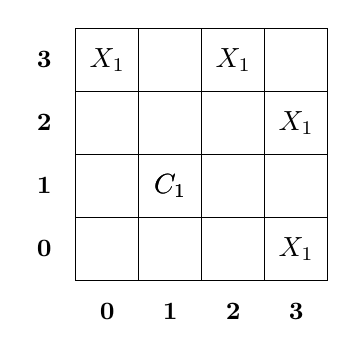
\begin{tikzpicture}[scale=0.8]
        % Dibuja el tablero
        \foreach \x in {0,1,2,3} {
            \foreach \y in {0,1,2,3} {
                \fill[white] (\x,\y) rectangle (\x+1,\y+1);
                \draw (\x,\y) rectangle (\x+1,\y+1);
            }
        }
    
        % Marcar los caballos con C_i
        \node at (1.5, 1.5) {$C_1$}; % (1,1)
    
        % Marcar las casillas alcanzables con X_i
        \node at (0.5, 3.5) {$X_1$}; % (0,3)
        \node at (1.5, 1.5) {$C_1$}; % (1,1)
        \node at (2.5, 3.5) {$X_1$}; % (2,3)
        \node at (3.5, 0.5) {$X_1$}; % (3,0)
        \node at (3.5, 2.5) {$X_1$}; % (3,2)
    
        % Etiquetas
        \foreach \x in {0,...,3} {
            \foreach \y in {0,...,3} {
                % Etiquetas de fila y columna
                \ifnum\x=0
                    \node at (-0.5,\y+0.5) {\textbf{\small \y}};
                \fi
                \ifnum\y=0
                    \node at (\x+0.5,-0.5) {\textbf{\small \x}};
                \fi
            }
        }
    \end{tikzpicture}
    \end{center}
    \item En otro caso se devuelve true pues todas las casillas son alcanzables (algunas por más de un caballo).
    \begin{center}
    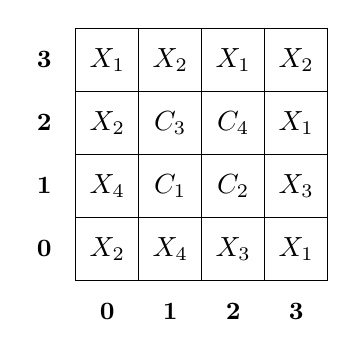
\begin{tikzpicture}[scale=0.8]
        % Dibuja el tablero
        \foreach \x in {0,1,2,3} {
            \foreach \y in {0,1,2,3} {
                \fill[white] (\x,\y) rectangle (\x+1,\y+1);
                \draw (\x,\y) rectangle (\x+1,\y+1);
            }
        }
        
        % Caballos en posiciones C_i
        \node at (1.5, 1.5) {$C_1$}; % (1,1)
        \node at (2.5, 1.5) {$C_2$}; % (2,1)
        \node at (1.5, 2.5) {$C_3$}; % (1,2)
        \node at (2.5, 2.5) {$C_4$}; % (2,2)
    
        % Marcar las casillas alcanzables con X_i
        \node at (0.5, 0.5) {$X_2$}; % (0,0)
        \node at (0.5, 1.5) {$X_4$}; % (0,1)
        \node at (0.5, 2.5) {$X_2$}; % (0,2)
        \node at (0.5, 3.5) {$X_1$}; % (0,3)
        \node at (1.5, 0.5) {$X_4$}; % (1,0)
        \node at (1.5, 3.5) {$X_2$}; % (1,3)
        \node at (2.5, 0.5) {$X_3$}; % (2,0)
        \node at (2.5, 3.5) {$X_1$}; % (2,3)
        \node at (3.5, 0.5) {$X_1$}; % (3,0)
        \node at (3.5, 1.5) {$X_3$}; % (3,1)
        \node at (3.5, 2.5) {$X_1$}; % (3,2)
        \node at (3.5, 3.5) {$X_2$}; % (3,3)
    
        % Etiquetas
        \foreach \x in {0,...,3} {
            \foreach \y in {0,...,3} {
                % Etiquetas de fila y columna
                \ifnum\x=0
                    \node at (-0.5,\y+0.5) {\textbf{\small \y}};
                \fi
                \ifnum\y=0
                    \node at (\x+0.5,-0.5) {\textbf{\small \x}};
                \fi
            }
        }
        
    \end{tikzpicture}
    \end{center}
\end{itemize}

\section{Dama amenazada}
Dado un tablero de ajedrez donde se ubican solo damas (reinas), determine si existe alguna que amenace a otra. La representación del tablero será un array bidimensional de bool donde solo habrá true en las casillas donde haya una reina.


\section{Jaque al rey}
Implemente un método que reciba un tablero de ajedrez, y determine si el rey negro está amenazado por alguna pieza blanca. 

El método deberá tener la siguiente signatura:

\begin{lstlisting}
    public enum ChessPiece
    {
        None,           // No piece (empty square)
        WhitePawn,
        WhiteKnight,
        WhiteBishop,
        WhiteRook,
        WhiteQueen,
        WhiteKing,
        BlackPawn,
        BlackKnight,
        BlackBishop,
        BlackRook,
        BlackQueen,
        BlackKing
    }
    
    public static bool IsBlackKingInCheck(ChessPiece[,] board)
    {
        // ...
    }
\end{lstlisting}


\section{Recorriendo islas}
El mapa de unas islas está modelado mediante un array bidimensional booleano, donde las casillas con valor true son secciones de tierra firme y las casillas con valor false son agua. Se desea encontrar cuál es la distancia mínima a recorrer entre el par de casillas \( (f_i, c_i) \) y \( (f_s, c_s) \) si solo se puede transitar por secciones de tierra firme.


\section{Tic-Tac-Toe}
Implementa un juego sencillo de Cerito-Cruz para dos jugadores.

\textbf{Requisitos:}
\begin{itemize}
    \item Usa un array bidimensional de 3x3 para representar el tablero.
    \item Los jugadores deben turnarse para colocar sus símbolos (\texttt{X} o \texttt{O}).
    \item Verifica si algún jugador ha ganado o si hay un empate.
\end{itemize}


% \section{Busca el Tesoro}
% \textbf{Descripción:}  
% Crea un juego donde el jugador debe encontrar un "tesoro" oculto en un tablero de tamaño 5x5.

% \textbf{Requisitos:}
% \begin{itemize}
%     \item Genera el tablero con celdas iniciales vacías (\texttt{-}).
%     \item Oculta el tesoro en una posición aleatoria.
%     \item Permite al jugador adivinar las coordenadas del tesoro.
%     \item Muestra un mensaje cuando el jugador encuentra el tesoro.
% \end{itemize}

% \textbf{Extensiones:}
% \begin{itemize}
%     \item Añade un contador de intentos.
%     \item Da pistas indicando si el tesoro está más cerca o lejos después de cada intento.
% \end{itemize}


% \section*{Ejercicio 4: Simulación de Ajedrez}
% \textbf{Descripción:}  
% Crea un programa que simule el movimiento de una pieza de ajedrez en un tablero de 8x8.

% \textbf{Requisitos:}
% \begin{itemize}
%     \item Representa el tablero como una matriz 8x8.
%     \item Permite al usuario elegir una pieza (torre, alfil, caballo).
%     \item Muestra los movimientos posibles desde una posición inicial ingresada por el usuario.
% \end{itemize}

% \textbf{Extensiones:}
% \begin{itemize}
%     \item Valida si un movimiento es válido para la pieza seleccionada.
%     \item Permite mover la pieza varias veces en el tablero.
% \end{itemize}


\section{El Mago y el Bosque Encantado}

En un bosque encantado, un mago ha decidido medir el poder de su hechizo de teletransportación. El bosque está representado como una cuadrícula de \(N \times M\), donde cada celda puede estar despejada o bloqueada por un obstáculo mágico. El mago comienza en una posición definida por el usuario, y desea calcular cuán lejos puede llegar su hechizo desde esa posición, sin atravesar los obstáculos.

\subsection*{Detalles del problema}

\begin{itemize}
    \item El bosque se representa como una matriz booleana: 
    \begin{itemize}
        \item \texttt{false}: La celda está despejada (el hechizo puede pasar).  
        \item \texttt{true}: La celda está bloqueada (el hechizo no puede pasar).  
    \end{itemize}
    \item La entrada incluye la posición inicial del mago \((x, y)\).  
    \item El resultado debe ser una matriz que indique la distancia desde la posición inicial hasta cada celda accesible, respetando los obstáculos. Las celdas bloqueadas deben marcarse como \(-1\) en la salida.  
\end{itemize}

\subsection*{Ejemplo}

\text{Entrada:}
\begin{itemize}
        \item Posición inicial del mago: \((2, 2)\).  
        \item Bosque: 
        \[ 
        \begin{bmatrix}
            \texttt{false} & \texttt{false} & \texttt{false} & \texttt{false} & \texttt{false} \\
            \texttt{false} & \texttt{false} & \texttt{false} & \texttt{true}  & \texttt{false} \\
            \texttt{false} & \texttt{false} & \texttt{false} & \texttt{false} & \texttt{false} \\
            \texttt{false} & \texttt{false} & \texttt{false} & \texttt{true}  & \texttt{false} \\
            \texttt{false} & \texttt{false} & \texttt{false} & \texttt{false} & \texttt{false} \\
            \end{bmatrix}
        \]
\end{itemize}

\text{Salida:}
\[
\begin{bmatrix}
4 & 3 & 2 & 3 & 4 \\
3 & 2 & 1 & -1 & 3 \\
2 & 1 & 0 & 1  & 2 \\
3 & 2 & 1 & -1 & 3 \\
4 & 3 & 2 & 3  & 4 \\
\end{bmatrix}
\]

\section*{Movimientos de las Piezas de Ajedrez}

\begin{itemize}
    \item \textbf{Peón (Pawn):}
    \begin{itemize}
        \item Avanza 1 casilla hacia adelante; 2 casillas si es el primer movimiento.
        \item Captura en diagonal hacia adelante.
        \item Movimientos especiales: \emph{en passant} y promoción al llegar al extremo del tablero.
    \end{itemize}

    \item \textbf{Caballo (Knight):}
    \begin{itemize}
        \item Se mueve en forma de "L" (2 casillas en una dirección, 1 en la otra).
        \item Puede saltar sobre otras piezas.
    \end{itemize}

    \item \textbf{Alfil (Bishop):}
    \begin{itemize}
        \item Se mueve cualquier número de casillas en las diagonales.
    \end{itemize}

    \item \textbf{Torre (Rook):}
    \begin{itemize}
        \item Se mueve cualquier número de casillas horizontal o verticalmente.
        \item Participa en el \emph{enroque} con el rey.
    \end{itemize}

    \item \textbf{Dama (Queen):}
    \begin{itemize}
        \item Combina los movimientos de la torre y el alfil: horizontal, vertical o diagonal.
    \end{itemize}

    \item \textbf{Rey (King):}
    \begin{itemize}
        \item Se mueve 1 casilla en cualquier dirección.
        \item Participa en el \emph{enroque} bajo ciertas condiciones.
    \end{itemize}
\end{itemize}


\section{Validación de un Sudoku}

En este ejercicio, implementarás un programa que valide si un tablero de Sudoku es válido. Un tablero de Sudoku debe cumplir con las siguientes reglas:

\begin{enumerate}
    \item Cada fila debe contener los números del \(1\) al \(9\) sin repetir.
    \item Cada columna debe contener los números del \(1\) al \(9\) sin repetir.
    \item Cada subcuadrícula de \(3 \times 3\) debe contener los números del \(1\) al \(9\) sin repetir.
\end{enumerate}

El programa recibirá como entrada un tablero representado como una matriz de \(9 \times 9\). Algunas celdas estarán vacías, representadas por un \(0\).

\subsection*{Ejemplo de entrada}
\[
\text{sudoku} = 
\begin{bmatrix}
5 & 3 & 0 & 0 & 7 & 0 & 0 & 0 & 0 \\
6 & 0 & 0 & 1 & 9 & 5 & 0 & 0 & 0 \\
0 & 9 & 8 & 0 & 0 & 0 & 0 & 6 & 0 \\
8 & 0 & 0 & 0 & 6 & 0 & 0 & 0 & 3 \\
4 & 0 & 0 & 8 & 0 & 3 & 0 & 0 & 1 \\
7 & 0 & 0 & 0 & 2 & 0 & 0 & 0 & 6 \\
0 & 6 & 0 & 0 & 0 & 0 & 2 & 8 & 0 \\
0 & 0 & 0 & 4 & 1 & 9 & 0 & 0 & 5 \\
0 & 0 & 0 & 0 & 8 & 0 & 0 & 7 & 9 \\
\end{bmatrix}
\]

\subsection*{Tareas}
\begin{enumerate}
    \item Implementa un método que valide cada fila para verificar que no haya duplicados.
    \item Implementa un método que valide cada columna para verificar que no haya duplicados.
    \item Implementa un método que valide cada subcuadrícula de \(3 \times 3\) para verificar que no haya duplicados.
    \item Implementa un método \texttt{isValidSudoku()} que combine las reglas anteriores y determine si el tablero de Sudoku es válido.
\end{enumerate}

\subsection*{Salida esperada}

\begin{itemize}
    \item Para el tablero de entrada anterior, el programa debe devolver:
    \[
    \text{El tablero de Sudoku es válido: Sí.}
    \]
    \item Si se modifica la celda \((1,2)\) del tablero para que contenga un \(5\), el programa debe devolver:
    \[
    \text{El tablero de Sudoku es válido: No.}
    \]
\end{itemize}

\subsection*{Extensiones del ejercicio}
\begin{enumerate}
    \item \textbf{Resolver el Sudoku:} Extiende el ejercicio para que, además de validar el tablero, puedas resolverlo. Usa técnicas como \textit{backtracking}.
    \item \textbf{Generar Sudokus:} Crea un generador de tableros de Sudoku que cumpla las reglas de validez.
    \item \textbf{Interfaz gráfica:} Diseña una interfaz gráfica para que el usuario pueda ingresar un tablero de Sudoku y verificarlo.
\end{enumerate}

\section{Validación de movimientos en Ajedrez}

Tu misión es implementar un programa en C\# que determine si un movimiento de una pieza de ajedrez es válido. Usarás el siguiente enumerado para representar las piezas:

\begin{lstlisting}[caption=Enumeración para las piezas de ajedrez]
public enum ChessPiece
{
    None,           // No piece (empty square)
    WhitePawn,
    WhiteKnight,
    WhiteBishop,
    WhiteRook,
    WhiteQueen,
    WhiteKing,
    BlackPawn,
    BlackKnight,
    BlackBishop,
    BlackRook,
    BlackQueen,
    BlackKing
}
\end{lstlisting}

El tablero se representará como una matriz de \(8 \times 8\) de tipo \texttt{ChessPiece}, donde cada celda indica la pieza presente o está vacía (\texttt{None}).

\subsection*{Descripción del problema}

Tu programa debe:
\begin{enumerate}
    \item Recibir como entrada:
    \begin{itemize}
        \item Un tablero \(8 \times 8\) inicializado con las piezas en su posición.
        \item Coordenadas iniciales y finales del movimiento: \((x_1, y_1)\) y \((x_2, y_2)\).
    \end{itemize}
    \item Determinar si el movimiento es válido según las reglas de la pieza en la posición inicial.
    \item Devolver si el movimiento es válido o no.
\end{enumerate}

\subsection*{Tareas}
\begin{enumerate}
    \item Implementa una función para validar movimientos básicos de cada tipo de pieza. Por ejemplo:
    \begin{itemize}
        \item Los peones solo avanzan (o retroceden, si son negros) una casilla, excepto al inicio.
        \item Los caballos se mueven en "L".
        \item Los alfiles solo se mueven en diagonal.
        \item Las torres solo se mueven en línea recta.
        \item Las reinas combinan los movimientos de las torres y los alfiles.
        \item Los reyes se mueven una casilla en cualquier dirección.
    \end{itemize}
    \item Valida si la celda destino está vacía o contiene una pieza del oponente.
    \item Devuelve si el movimiento cumple las reglas de la pieza.
\end{enumerate}

\subsection*{Ejemplo de entrada}

\begin{lstlisting}[caption=Tablero inicial]
ChessPiece[,] board = new ChessPiece[8, 8]
{
    { ChessPiece.BlackRook, ChessPiece.BlackKnight, ChessPiece.BlackBishop, ChessPiece.BlackQueen, ChessPiece.BlackKing, ChessPiece.BlackBishop, ChessPiece.BlackKnight, ChessPiece.BlackRook },
    { ChessPiece.BlackPawn, ChessPiece.BlackPawn, ChessPiece.BlackPawn, ChessPiece.BlackPawn, ChessPiece.BlackPawn, ChessPiece.BlackPawn, ChessPiece.BlackPawn, ChessPiece.BlackPawn },
    { ChessPiece.None, ChessPiece.None, ChessPiece.None, ChessPiece.None, ChessPiece.None, ChessPiece.None, ChessPiece.None, ChessPiece.None },
    { ChessPiece.None, ChessPiece.None, ChessPiece.None, ChessPiece.None, ChessPiece.None, ChessPiece.None, ChessPiece.None, ChessPiece.None },
    { ChessPiece.None, ChessPiece.None, ChessPiece.None, ChessPiece.None, ChessPiece.None, ChessPiece.None, ChessPiece.None, ChessPiece.None },
    { ChessPiece.None, ChessPiece.None, ChessPiece.None, ChessPiece.None, ChessPiece.None, ChessPiece.None, ChessPiece.None, ChessPiece.None },
    { ChessPiece.WhitePawn, ChessPiece.WhitePawn, ChessPiece.WhitePawn, ChessPiece.WhitePawn, ChessPiece.WhitePawn, ChessPiece.WhitePawn, ChessPiece.WhitePawn, ChessPiece.WhitePawn },
    { ChessPiece.WhiteRook, ChessPiece.WhiteKnight, ChessPiece.WhiteBishop, ChessPiece.WhiteQueen, ChessPiece.WhiteKing, ChessPiece.WhiteBishop, ChessPiece.WhiteKnight, ChessPiece.WhiteRook }
};
\end{lstlisting}

Movimiento a validar:
\[
(x_1, y_1) = (6, 4), \quad (x_2, y_2) = (5, 4)
\]

\subsection*{Salida esperada}

\[
\text{Movimiento válido.}
\]

\subsection*{Extensiones del ejercicio}
\begin{itemize}
    \item Valida movimientos especiales como:
    \begin{itemize}
        \item Enroque.
        \item Captura al paso (\textit{en passant}).
        \item Promoción de peones.
    \end{itemize}
    \item Determina si un movimiento pone al rey propio en jaque y evítalo.
\end{itemize}
